\chapter{Klassen en objecten in C++} \label{chap:klas}
Als eerste wordt er verbinding gemaakt vanaf je laptop met de RockPi, waarna een LEDje aan- en uitgezet wordt. Vervolgens wordt door middel van een programma een aantal LEDs aangestuurd.

\begin{comment}
Het practicum wordt gedaan op een RockPi dit is een single board computer dat draait in ons geval met het linux operating systeem. Met behulp van de RockPi wordt tijdens het practicum door middel van objecten diverse LEDs aangestuurd. Dit wordt gedaan door een 1 of een 0 naar naar een file te schrijven. In Figuur \ref{fig:netw} wordt weergegeven hoe de RockPi op het lab netwerk is aangesloten.
\begin{figure}[h!]
	\centering
	\begin{center} 	
			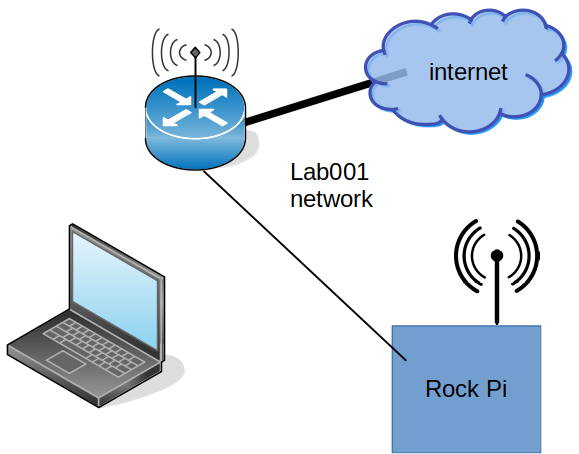
\includegraphics[width=0.4\textwidth]{figuren/laBnetwork}
			\caption{De rockPi in het lab-netwerk}
      	\label{fig:netw}   
	\end{center}
\end{figure}
Dit kan via de lab-wifi of via een UTP kabel. Het bijbehorende Ipnr. wordt getoond op het 
displaytje dat aangesloten is op de RockPi. Om contact te kunnen maken tussen de laptop en de RockPi moet de laptop \textbf{ook} op het \textbf{labnetwerk(Lab001) aangesloten} zijn, b.v. via de wifi.


\section{De eerste kennismaking met de RockPi.}

\end{comment}

\section{Werken met de RockPi.}

\subsection{Verbinding opzetten met de RockPi}\label{chp:contactPi}

In eerste instantie wordt er verbinding gemaakt met de RockPi via het \textit{ssh} commando.
\begin{figure}[h!]
	\centering
	\begin{center} 	
		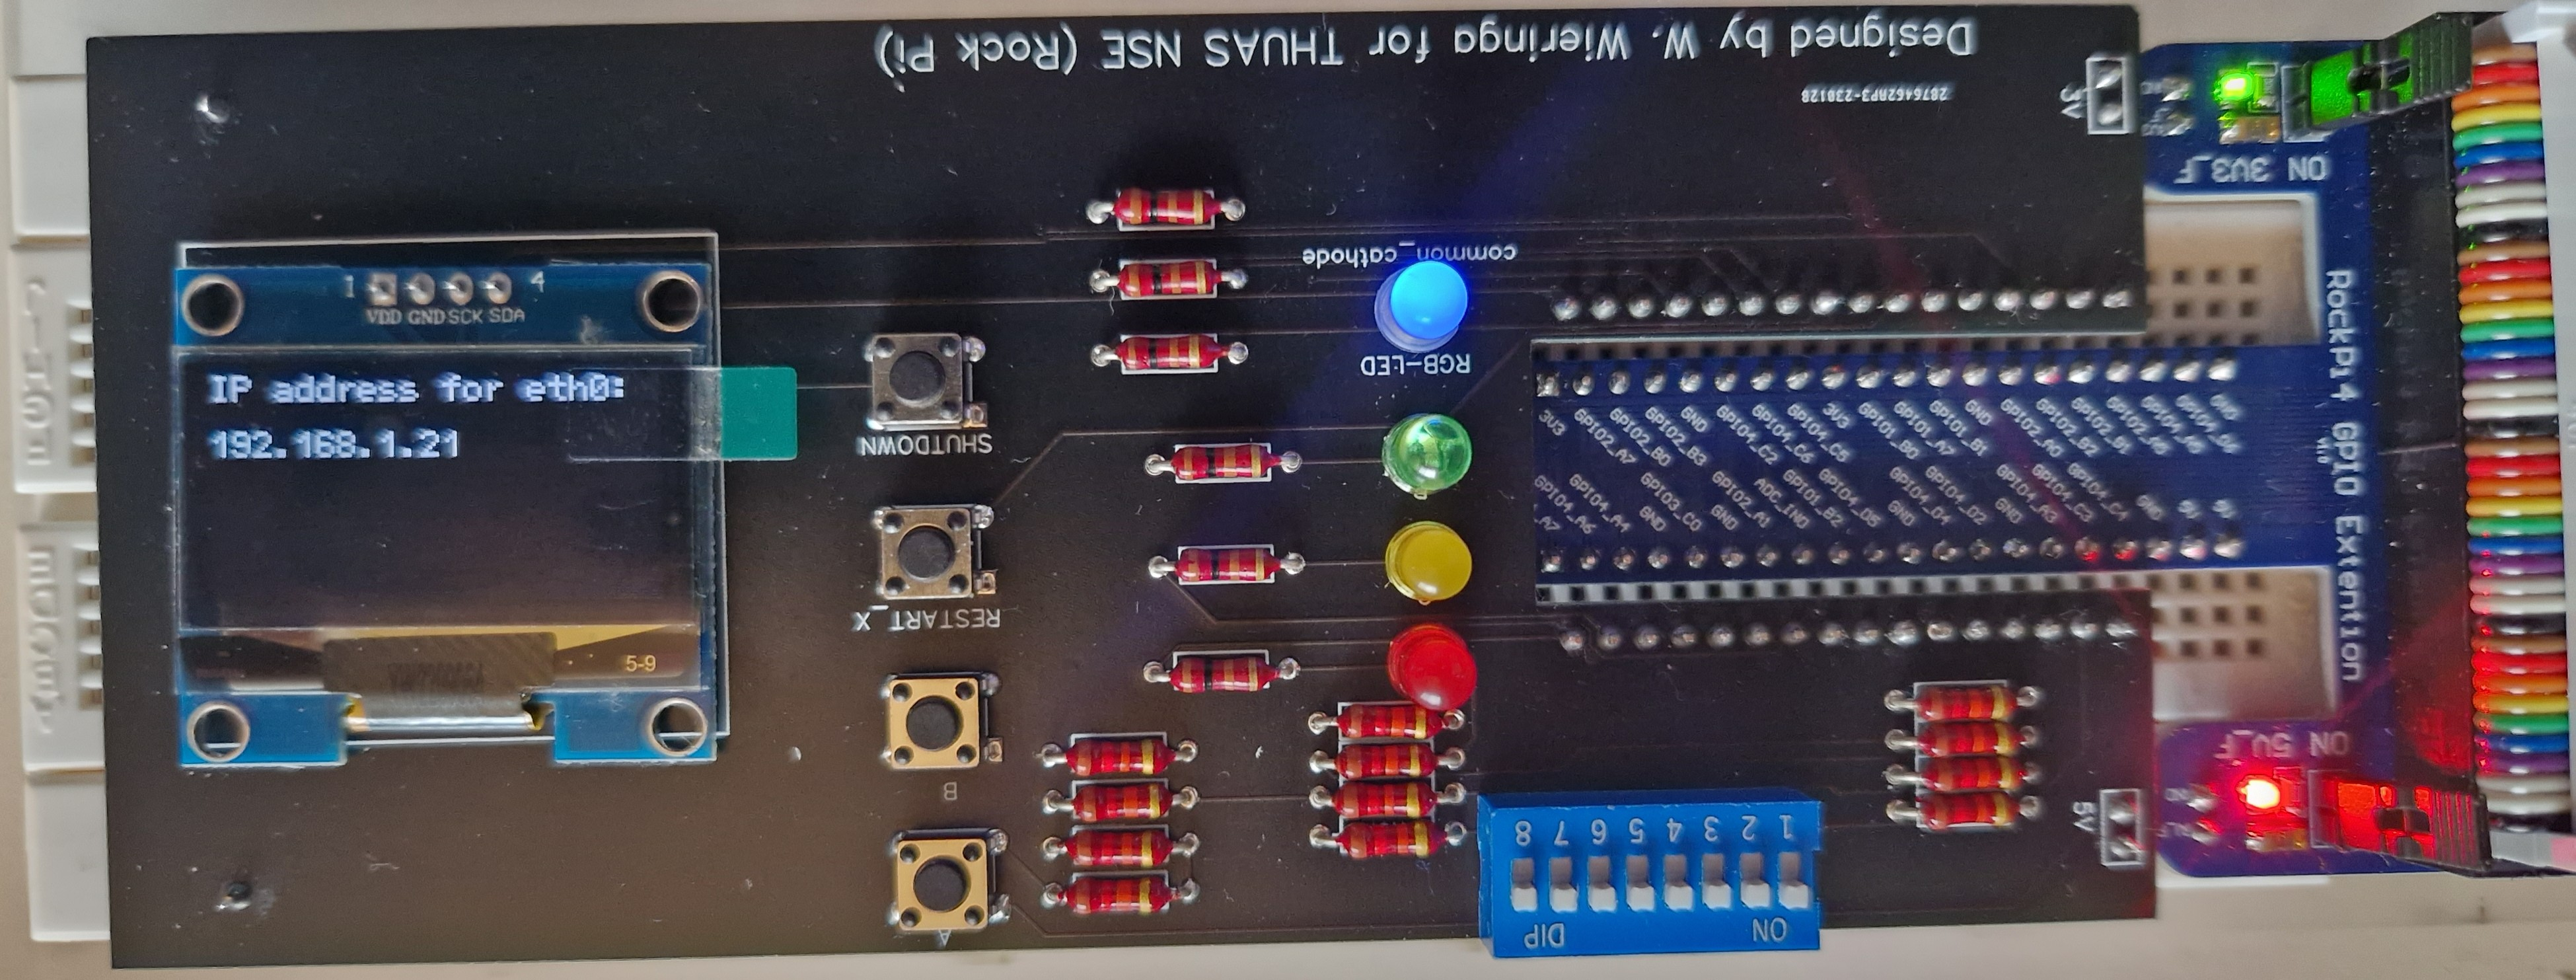
\includegraphics[width=1\textwidth]{figuren/rockIPnr}
		\caption{De RockPi met het \textit{IP adres.}}
		\label{fig:rockpiip}   
	\end{center}
\end{figure}
 Het IP adres van de RockPi is af te lezen via het oled display zoals in Figuur \ref{fig:rockpiip} wordt weergegeven. In het voorbeeld hierna wordt het IP adres \textit{192.168.178.89} gebruikt.


Open in Windows een terminal (b.v. een PowerShell, cmd prompt of een extern programma zoals b.v. \href{https://www.fosshub.com/KiTTY.html}{KiTTY}). We gebruiken voor nu PowerShell: Ga naar Windows Search: druk Windows+S (de knop met het Windows vlaggetje + de 'S'), zie Figuur \ref{fig:windowsZk} en
\begin{figure}[h!]
	\centering
	\begin{center} 	
		%\begin{subfigure}[b]{0.63\textwidth}
			
\includegraphics[width=1\textwidth]{figuren/windowsPowerShellSearch}
			\caption{Zoekscherm in Windows}
			\label{fig:windowsZk}
		%\end{subfigure}
	\begin{comment}
		\begin{subfigure}[b]{0.63\textwidth}
			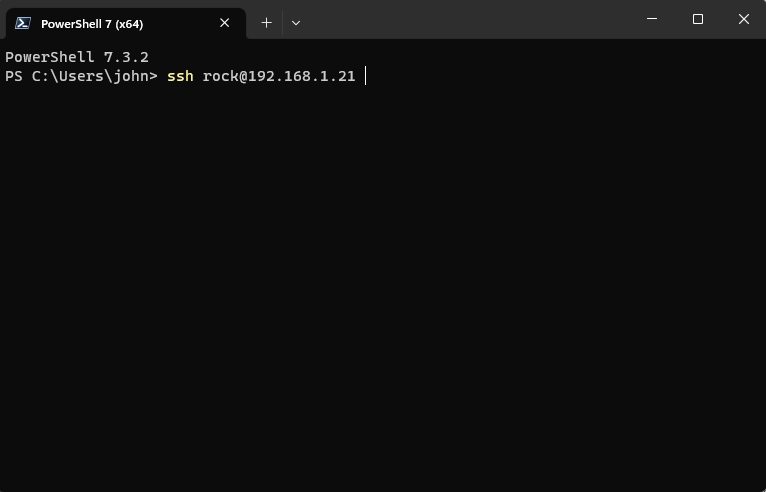
\includegraphics[width=1\textwidth]{figuren/powershell}
			\caption{ssh verbinding maken naar de RockPi }
			\label{fig:sshPi}
		\end{subfigure}
		\caption{Opstelling bij opdracht 1.}
		\label{fig:contactPi}   
	\end{comment}
	\end{center}
\end{figure}
tik vervolgens in: \textit{powershell}. In de PowerShell kan het \textit{ssh} commando met de username en het IP adres gegeven worden, zoals in Figuur \ref{fig:rockpiLogIn} wordt weergegeven. Bij de eerste keer zal de melding komen of de host key moet worden opgeslagen, kies \textit{yes}. Vervolgens zal om om het password gevraagd worden. Dit is \textit{rock}. 

\clearpage
Wanneer het inloggen gelukt is, verschijnt een verhaaltje dat eindigt met de prompt van de RockPi, zoals in Figuur \ref{fig:rockpiLogIn} te zien is.
\begin{figure}[h!]
	\centering
	\begin{center} 	
		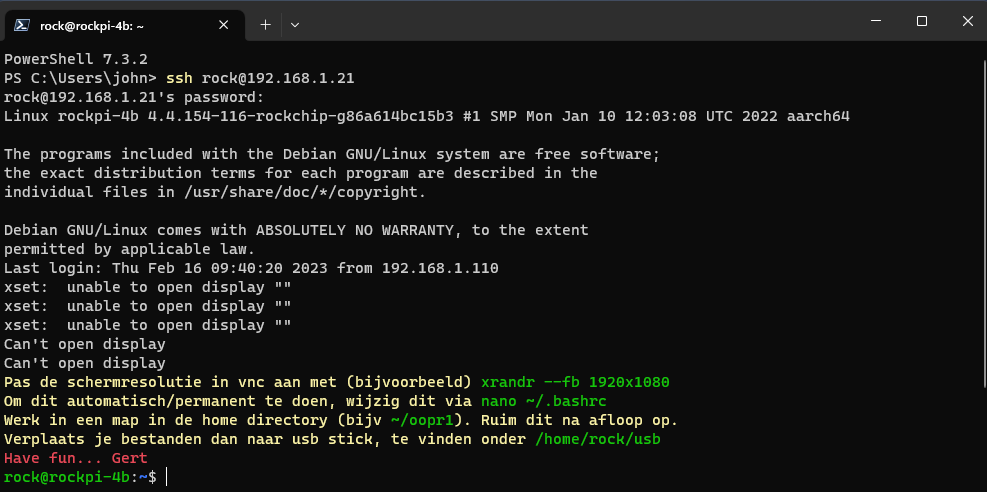
\includegraphics[width=1\textwidth]{figuren/ingelogtRockPi}
		\caption{Ingelogd in de RockPi}
		\label{fig:rockpiLogIn}   
	\end{center}
\end{figure}
Vanaf nu werk je in een Linux terminal omgeving. Een listing van een directory kan opgevraagd worden met het \textit{ls} commando (list files and directories), het veranderen van een directory kan gedaan worden het \textit{cd} commando (change directory) en het maken van een directory met het \textit{mkdir}  commando (make directory). Verdere Linux commando's en tips zijn te vinden in  \hyperlink{LinuxTipsTrics}{de Bijlage}.

\clearpage
\subsection{Het aansturen van een LED.}
Wanneer contact is gemaakt met de RockPi, zoals beschreven in hoofdstuk \ref{chp:contactPi}, kunnen de LEDs aangestuurd worden. De LED's zitten aangesloten op de GPIO ('General Purpose Input Output') connector van de RockPI, deze is te zien in Figuur \ref{fig:rockpiCon}.
\begin{figure}[h!]
	\centering
	\begin{center} 	
		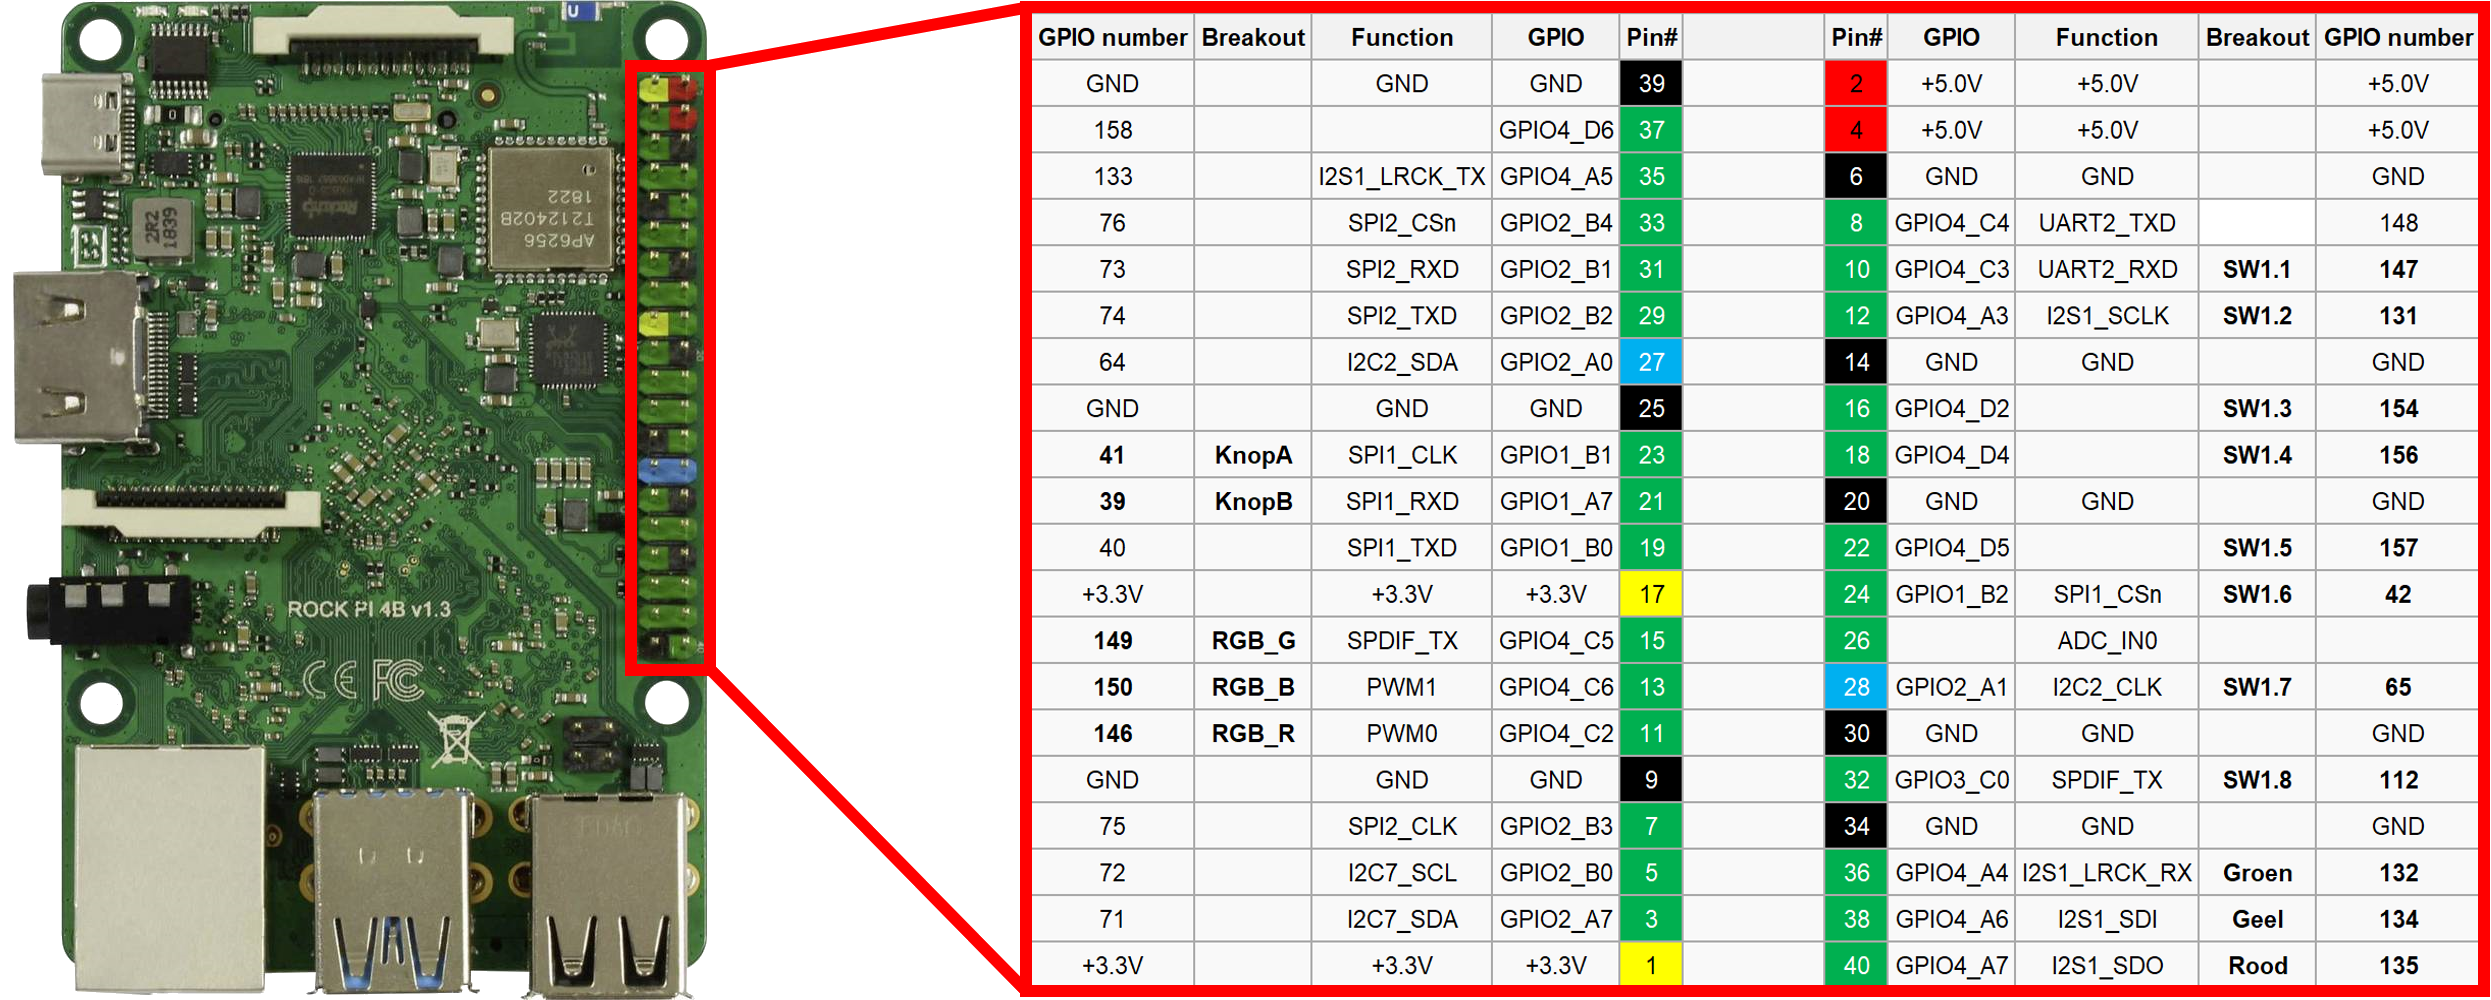
\includegraphics[width=1.1\textwidth]{figuren/rockpi-connector}
		\caption{GPIO connector van de RockPI}
		\label{fig:rockpiCon}   
	\end{center}
\end{figure}
De buitenste kolom geeft het GPIO nummer aan waarop deze geprogrammeerd kan worden. Zo zit de rode LED aangesloten op GPIO nummer 135. De \textbf{dikgedrukte} pinnen worden gebruikt met de printplaat. In de kolom \textbf{breakout} zie je wat op die pinnen zit.

\paragraph[Opdracht 1a]{Opdracht 1a, het eerste programmaatje op de RockPi}	

\begin{enumerate}
	\item Plaats de \hyperlink{chp:USBstick}{USB stick} in de RockPi.
	\item Ga naar de directory van je USB stick
	\begin{itemize}
		\item \textit{cd Documents} (het hele pad is \textit{/media/rock/Documents} )
	\end{itemize}
    
    \item Maak een directory \textit{ledje} aan en ga daar na toe.
	\begin{itemize}
	    \item \textit{mkdir ledje}
	    \item \textit{cd ledje}
    \end{itemize}  
   \item Download files \textit{gpiofuncties.h}, \textit{gpiofuncties.cpp}, \textit{test.cpp} van Github. Het main programma (\textit{test.cpp}) wordt in Listing \ref{lst:mainLd} weergegeven
   	\begin{itemize}
     	\item \textit{git clone https://github.com/JohnVi-hhs/oop.git}
     	\item \textit{cd oop}
     	\item \textit{ls -l}
     	\item \textit{nano test.cpp} Druk Ctrl+X om nano weer te sluiten.
   \end{itemize}

\clearpage
\begin{figure}[h!]
	\centering
	\begin{center} 	
		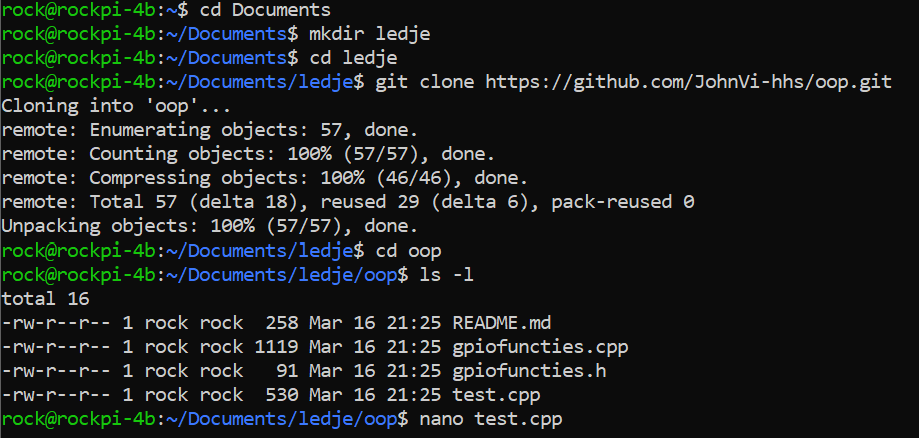
\includegraphics[width=0.94\textwidth]{figuren/gitclone}
		\caption{Schermuitvoer na bovenstaande opdrachten}
		\label{fig:gitclone}   
	\end{center}
\end{figure}

\begin{lstlisting}[caption=Zet LED aan en uit,frame=tlrb,label={lst:mainLd}]{Name}
#include <unistd.h>
#include <iostream>
#include "gpiofuncties.h"
	
using namespace std;
#define RODELED 135
	
int main() {
		
	cout<<"Hi NSE"<<endl;
	int b=zetPinOpOutput(RODELED);//return waarde of het gelukt is.
	if(b == 0)  {  //if(!b) mag ook. 
		cout<<"Foutje bedankt"<<endl;
		return 0;
	}
	cout<<"b= "<<b<<endl;//return waarde of het gelukt is.
	b=zetPinWaarde(RODELED,1);  //Zet de rode LED aan.
	usleep(1000000);
	b=zetPinWaarde(RODELED,0);  //Zet de rode LED uit.
	cout<<"einde"<<endl;
}
\end{lstlisting}
   \item Compileer en run het testprogramma.
\begin{itemize}
	\item Compileren van het programma. \\\textit{g++ -g3 *.cpp -o tst}\\
	optie \textit{-g3} heeft te maken met debug mogelijkheden. \\
	Optie \textit{-o} geeft een naam aan de output file (\textit{tst})
	\item Voer het zojuist gecompileerde programma tst uit.\\\textit{./tst}  
	
\end{itemize}
Resultaat:\\	
De rode LED gaat 1 seconde aan.

\item Pas het programma zodanig aan, zodat eerst de groene LED aangaat, daarna de gele LED en vervolgens de rode LED. \\
In de linux terminal, kunnen verschillende editors gebruikt worden, waarvan \href{https://linuxize.com/post/how-to-use-nano-text-editor/}{nano} \'{e}\'{e}n van de meest gebruikte is, een ander beroemde/beruchte editor is \href{https://opensource.com/article/19/3/getting-started-vim}{vim}  
Als je nano gebruikt: druk Ctrl+O om op te slaan en Ctrl+X om af te sluiten. Bij vim, druk/tik \textit{:help}
\end{enumerate}

\section{Het werken vanuit Visual Studio Code}

Hierbij wordt vanuit 'Visual Studio Code' (VSC) gewerkt, en wordt de klasse Led geïmplementeerd. Er wordt vanuit gegaan dat VSC geïnstalleerd is zoals in appendix  \ref{app:vsc} beschreven staat.  
\begin{enumerate}
	\item Start VSC op en maak verbinding met de RockPi.
	\begin{itemize}
		\item Klik op remote Explorer \img{figuren/remoteExplorer}. De IP nummers van de remote system(en) die al eerder gebruikt zijn worden zichtbaar, zoals te zien is in Figuur \ref{fig:remNr}. Als dit niet zo is, klik dan op \textcolor{red}{[1]} om de lijst te verversen, als je een nieuw systeem wilt toevoegen, klik \textcolor{red}{[2]}.
		\begin{figure}[h!]
			\centering
			\begin{center} 	
				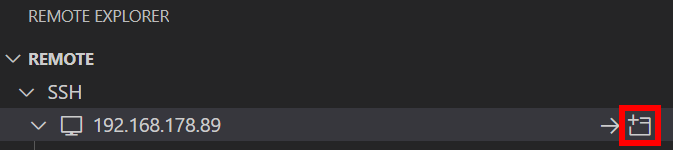
\includegraphics[width=0.8\textwidth]{figuren/remoteExplorer2}
				\caption{Remote Explorer van VSC}
				\label{fig:remNr}   
			\end{center}
		\end{figure}
				 
		\item  Maak nu verbinding met de RockPi door te klikken op \textcolor{red}{[3]} of \textcolor{red}{[4]}\newline
		(\textcolor{red}{[3]} = in hetzelfde venster), \textcolor{red}{[4]} = nieuw venster).

      \end{itemize}
      
      \item Nadat een verbinding gemaakt is met de RockPi, open een remote folder door op \img{figuren/VSCiconeExpl} te klikken (of druk \textbf{Ctrl+K} \textbf{Ctrl+O}) en ga naar de directory van de vorige opdracht: \texttt{/home/rock/Documents/ledje/oop/} \newline
      Aan de linkerkant worden de files zichtbaar en onderaan een statusbalk met informatie. Dit is te zien in Figuur \ref{fig:vncOp}
  		\begin{figure}[h!]
  	\centering
  	\begin{center} 	
  		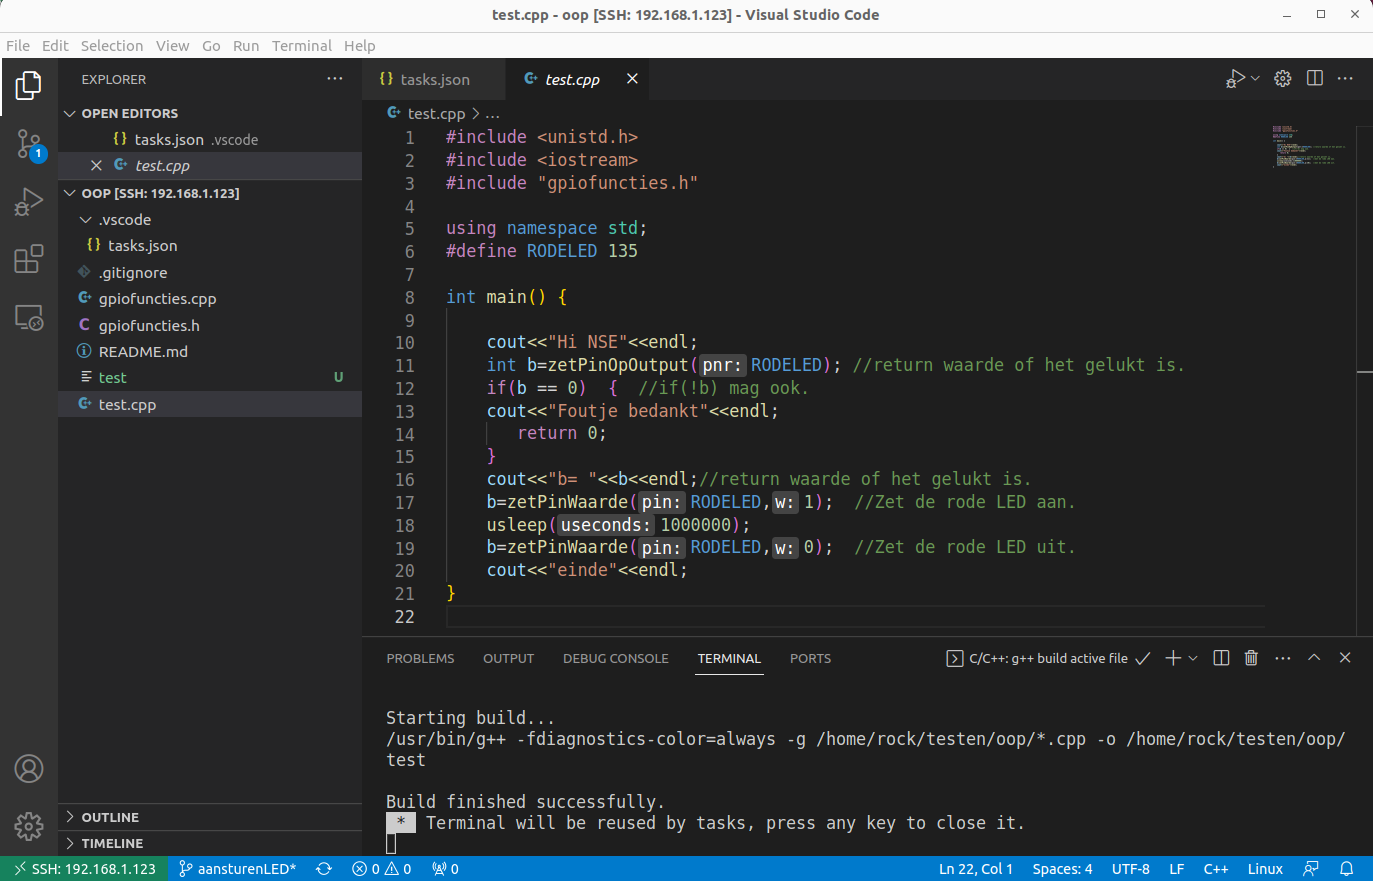
\includegraphics[width=0.72\textwidth]{figuren/vncSchermOp1}
  		\caption{VSCode in de gewenste directory}
  		\label{fig:vncOp}   
  	\end{center}
  \end{figure}    

\newpage
Klik op select folder  % Gert: Ik kan niks vinden wat 'select folder' heet
en selecteer de folder waarin de files staan. 


\begin{itemize}
	\item Selecteer in het 'Explorer' paneel de file \textit{test.cpp} en compileer de files\footnote{Compileren lukt niet: Controleer of de C++ extension (\img{figuren/cPlusIcon}) is geïnstalleerd en is geactiveerd.} (Terminal $\rightarrow$ Run Build Task... of \textbf{Ctrl+Shift+B}). \textit{(Als je rechtsonder in het venster een melding krijgt over CMake, klik deze dan weg, we gebruiken geen CMake.)}
	\item Klik links van regelnummer 10, er verschijnt een rood bolletje, dit is een breakpoint.
	\item Start het Debuggen: druk \textbf{F5} of selecteer bij het pijltje rechtsboven \img{figuren/debugPijl} de Debug optie en klik op de pijl (of Run $\rightarrow$ Start Debugging), De debugger wordt gestart en een scherm als in Figuur \ref{fig:debugScherm} verschijnt. (\textit{Als je een foutmelding krijgt: zorg dat je scherm eruit ziet als in Figuur \ref{fig:vncOp} en probeer opnieuw Debug te starten.})
	\begin{figure}[h!]
		\centering
		\begin{center} 	
			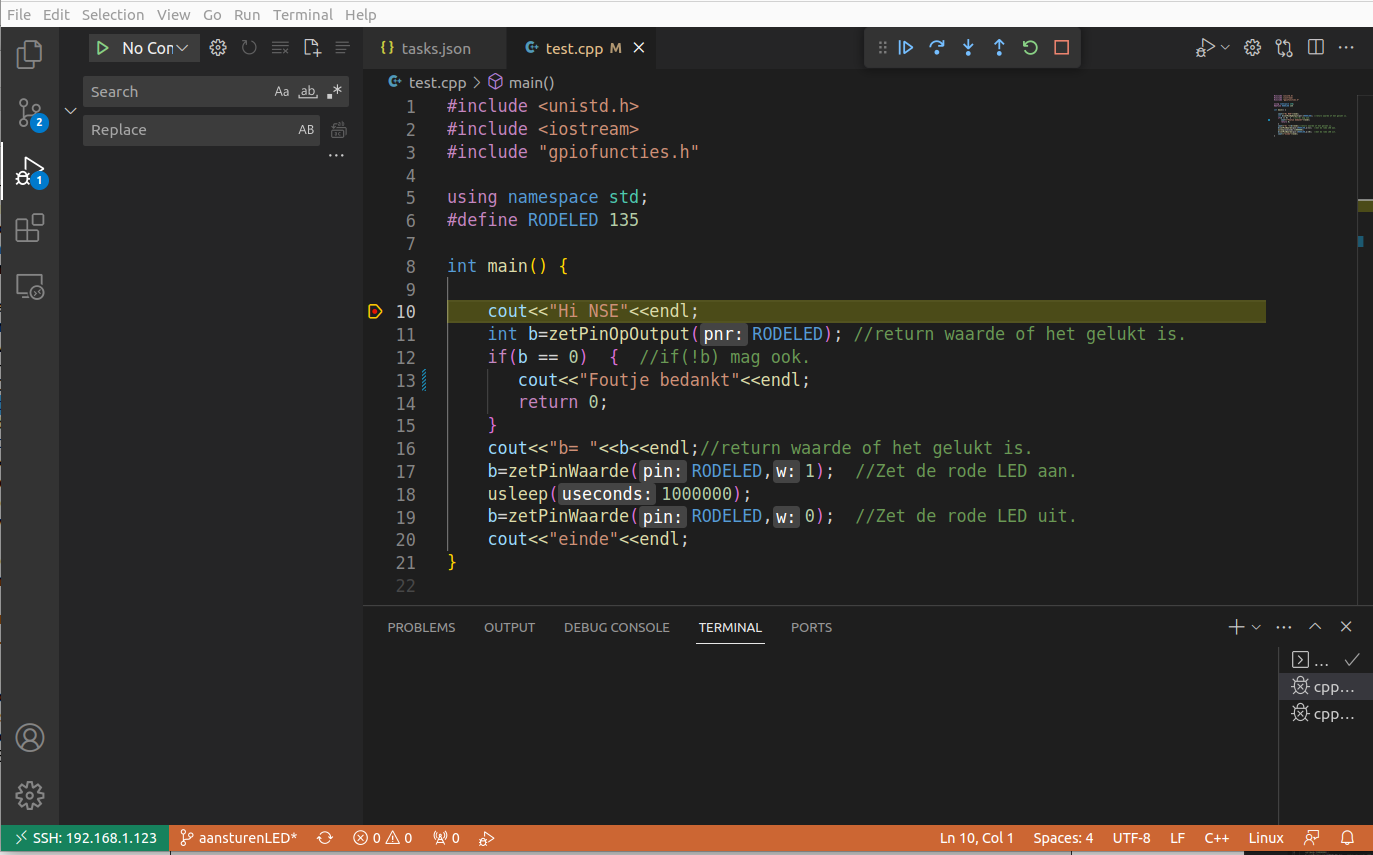
\includegraphics[width=1\textwidth]{figuren/debugScherm} % was 0.9
			\caption{Start van de debug sessie.}
			\label{fig:debugScherm}   
		\end{center}
	\end{figure}
	
	Met de debugknoppen rechtsboven kan nu stap voor stap het programma doorlopen worden (\hyperlink{chp:debugknoppen}{naar uitleg}, druk \textbf{Alt+$\leftarrow$} om hier terug te komen).\\
	Doorloop het programma stap voor stap met 'Step Over' (\textbf{F10}), zodat de LED ook daadwerkelijk bij een stap aan- en uitgaat. 
\end{itemize}

\item Bij deze opdracht wordt de eerste klasse gemaakt.
\begin{itemize}
	\item Maak een nieuwe terminal aan (Terminal $\rightarrow$ New Terminal of \textbf{Ctrl+Shift+`}) en maak een nieuwe directory aan:\\ \texttt{mkdir $\sim$/Documents/opdrLedH} gevolgd door \texttt{cd $\sim$/Documents/opdrLedH}
	\item clone de volgende code:\\
	 {\small \texttt{git clone } \verb|--|\texttt{branch opdrLedH https://github.com/JohnVi-hhs/oop.git}}
	 \item Sluit in VSC de huidige folder (\textbf{Ctrl+K F}) en open de folder\\ \texttt{/home/rock/Documents/opdrLedH/oop/}
	\item De UML notatie van de klasse \textbf{Led} wordt weergegeven in Figuur \ref{fig:klassLed} en de headerfile in listing \ref{lst:ledH}

	\begin{minipage}{0.5\textwidth} 
	\begin{figure}[H]
	%	\caption{\label{fig:label} Figure title}
		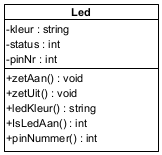
\includegraphics[width=0.9\textwidth]{figuren/klasseLedOpg1}
		\caption{UML diagram van de \\klasse Led}
		\label{fig:klassLed}   
	\end{figure}
\end{minipage}\hfill
\begin{minipage}{.45\textwidth}
	\begin{lstlisting}[caption=LED declaratie file(.h),frame=tlrb,label={lst:ledH}]{Name}
class Led
{
	public:
    	Led(int);
		Led(int, string);
		Led(int, string,string);
		~Led();
		void zetAan();
		void zetUit();
		string ledKleur()const;
		int isLedAan()const;
		int pinNummer() const;
		string deEigenaar() const;
			
	private:
		string kleur;
		int pinNr;
		int status;  
		string eigenaar;
};
		
		
	\end{lstlisting}
	
\end{minipage}

\newpage	
\paragraph{Opdracht:} Implementeer de Led.cpp zodat het hoofdprogramma van listing \ref{lst:hfdprg2} zonder errors en warning gecompileerd en uitgevoerd kan worden. 
\begin{lstlisting}[caption=Hoofdprogramma om de LED uit te testen ,frame=tlrb, label={lst:hfdprg2}]{Name}
#include <unistd.h>
#include <iostream>
#include <string>
#include "Led.h"

using namespace std;
#define RODELED 135
#define GROENELED 132
#define GELELED 134

int main() {
	
	cout<<"Hi NSE"<<endl;
	Led rood(RODELED,"Rood","Pietje Puk");
	Led geel(GELELED,"Geel");
	Led groen(GROENELED);
	
	groen.zetAan();
	usleep(1000000);
	groen.zetUit();
	geel.zetAan();
	usleep(1000000);
	geel.zetUit();
	rood.zetAan();
	usleep(1000000);  
	rood.zetUit();
	
	cout<<"einde"<<endl;
}

\end{lstlisting}	
\end{itemize}
\end{enumerate}

\paragraph{Opdracht:}
We gaan hierbij stap voor stap het programma doorlopen (debuggen), waarbij de inhoud van de objecten van de klasse Led wordt getoond.

\begin{enumerate} [label=\alph*]
	\item We laten je dit nu eerst in VSC zien, in het volgende hoofdstuk doen we hetzelfde met de DDD debugger.
	\begin{enumerate} [label=\roman*]
		
		\item Zet een breakpoint op regel 13, de regel met \texttt{\textit{Led rood(RODELED,"Rood", "Pietje Puk");}} Als het goed is staat nu vóór de 13 een rood bolletje.
		
		\item Zorg dat in het 'Explorer' paneel \textit{test.cpp} is geselecteerd. \\Start nu het debuggen (druk \textbf{F5}). Het programma wordt uitgevoerd tot het breakpoint.  Er verschijnt een pijl over het breakpoint. 
		\item In het linker paneel bovenaan zie je 'VARIABLES' met daaronder de locale variabelen. Klap 'rood' en 'geel' open, je kijkt nu naar gedeclareerde- maar nog niet-geïnitialiseerde objecten.
		\item Klik/druk op 'Step Over' \textbf{(F10)}. Regel 13 wordt uitgevoerd. 
		\\ Beantwoord: Wat zie je bij 'rood' veranderen? \\
		De pijl komt voor de regel \textit{Led geel(GELELED,"Geel");} te staan.
		\item Klik/druk op 'Step Into' \textbf{(F11)}, met dit commando wordt naar de constructor van de klasse Led gestapt. 
		\item Nu zie je links bij 'VARIABLES' andere variabelen; \textit{pin} en \textit{kleur}. \\Beantwoord: Waar komt de waarde van deze variabelen vandaan?
		\item Klik 'this' open en druk 'Step Over' \textbf{(F10)}.  \\(\textit{TIP}: Zorg dat er een commando in de constructor staat.) 
		\\Beantwoord: Wat zie je in/onder 'this' veranderen? Waardoor komt dat?
		\item Doorloop het programma verder stap voor stap; experimenteer met 'Step Over' \textbf{(F10)}, 'Step Into' \textbf{(F11)} en 'Step Out' \textbf{(Shift+F11)}
    \end{enumerate}
\end{enumerate}


\section{Het werken met de DDD visuele debugger.} \label{sec:startDDD}
 
Bij dit onderdeel van de opdracht wordt gewerkt met een grafische debugger. Hiermee wordt een grafische weergave gedaan wat een object is en wat een object van een afgeleide klasse inhoudt (dit laatste komt in opgave 2 aan de orde). Verder worden de associaties tussen objecten duidelijk weergegeven (dit wordt in week 4 en 5 gedaan).

De grafische debugger die gebruikt wordt is de DDD debugger (Data Display Debugger) 


Een paar handige links hierbij zijn:

\begin{itemize}
	\item DDD manual in \href{https://www.gnu.org/software/ddd/manual/html_mono/ddd.html}{html} en \href{https://www.gnu.org/software/ddd/manual/pdf/ddd.pdf}{pdf}
	\item \href{https://www.gnu.org/software/ddd/}{GNU DDD project}
	\item \href{href="https://taufanlubis.wordpress.com/2019/02/19/gnu-debugger-front-end-graphical-user-interface-with-ddd}{taufanlubis.wordpress.com}
	\item  \href{https://www.cs.swarthmore.edu/~newhall/unixhelp/howto_gdb.php}{Swarthmore}
	\item  \href{http://www.linuxfocus.org/English/January1998/article20.html}{linuxfocus}
\end{itemize}

\begin{comment}
De instellingen van de DDD debugger staan in de folder \texttt{.ddd} die staat in de home directory (\textit{/home/rock}). Soms is het eenvoudiger om deze directory te deleten dan de instellingen aan te passen (tips: \texttt{ls -al $\sim$} en \texttt{rm -rf $\sim$/.ddd}).
\end{comment}

We gaan nu met de DDD debugger werken.
Om met DDD te kunnen werken hebben we een grafische omgeving nodig. Een handige methode is om de de VNC viewer van de host te gebruiken. Deze viewer toont de grafische uitvoer van de RockPi. Open in de VNC een terminal, ga naar de directory die in de vorige opdracht gemaakt is (waar de files test.cpp, Led.cpp en Led.h \textcolor{green}{test} staan) en start de DDD debugger op:
\texttt{\textit{ddd test}}, vervolgens wordt het scherm, zoals weergegeven in Figuur \ref{fig:dddscherm1}, getoond.
\begin{figure}[h!]
	\captionsetup{justification=centering}
	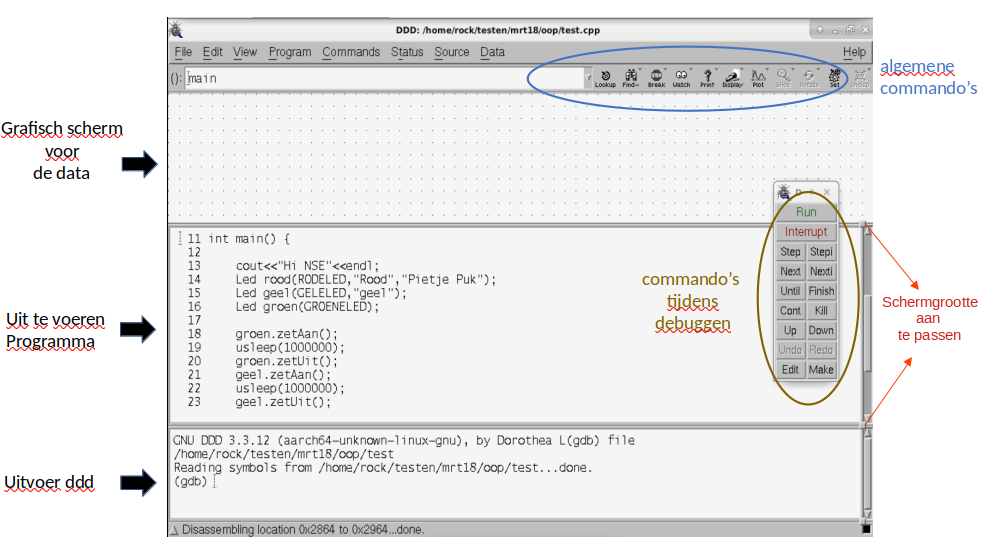
\includegraphics[width=0.8 \linewidth]{figuren/ddd_startup_screen}
	\centering
	\caption{het DDD opstartscherm.}
	\label{fig:dddscherm1}
\end{figure}

\paragraph{Opdracht:}
We gaan hierbij stap voor stap het programma doorlopen, waarbij de inhoud van de objecten van de klasse Led wordt getoond.

\begin{enumerate} [label=\alph*]
	\item Als eerste een korte kennismaking met de DDD debugger.
\begin{enumerate} [label=\roman*]

	\item Zet de cursor op de regel \texttt{\textit{Led rood(RODELED,"Rood", "Pietje Puk");}}
	(regelnummer 13)
	\item Klik op \textit{Break} (bij `algemene commando's`, zie Figuur \ref{fig:dddscherm1}). Voor het begin van de regel verschijnt nu een breakpoint (een rood STOP-bordje).

\begin{figure}[h!]
	\captionsetup{justification=centering}
	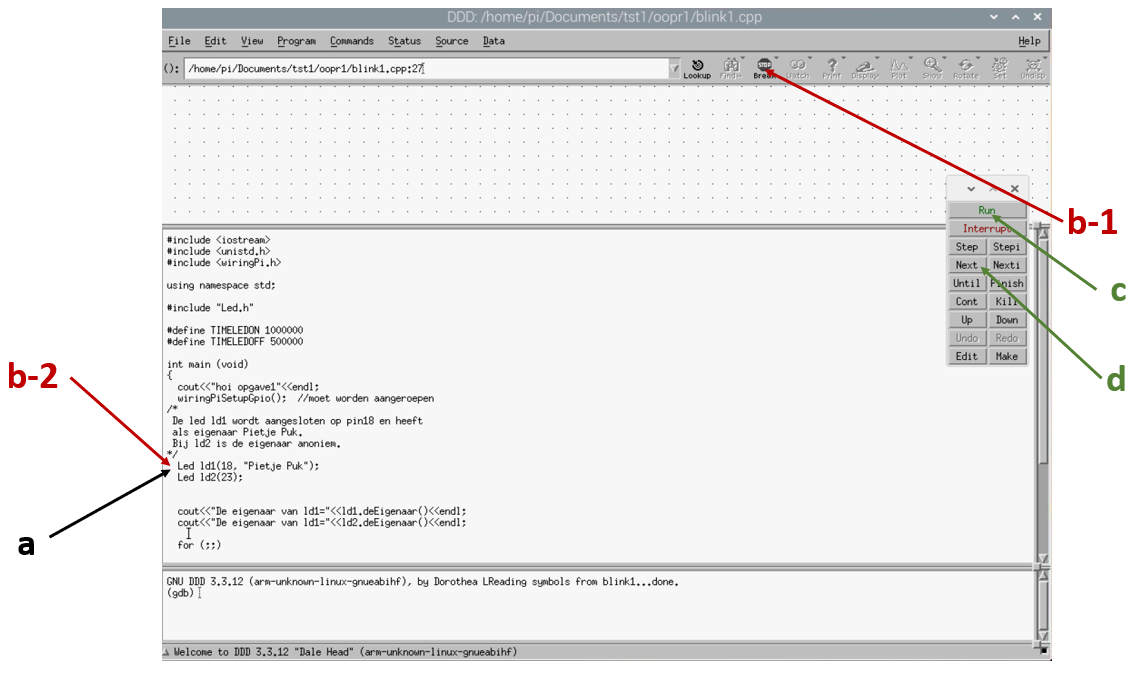
\includegraphics[width=0.7 \linewidth]{figuren/ddd_set_breakpoint}
	\centering
	\caption{het zetten van een breakpoint.}
	\label{fig:ddduitv1}
\end{figure}
	\item Klik op \textit{Run} (bij `commando's tijdens debuggen`),
het programma wordt uitgevoerd tot het breakpoint. \\Er verschijnt een groene pijl voor het breakpoint.
\item Klik op \textit{Next}, de regel wordt uitgevoerd (dit doet hetzelfde als de `step over` bij VSC). \\
De groene pijl komt voor de regel \textit{Led geel(GELELED,"Geel");} te staan. 
\item Klik op \textit{Step}, met dit commando wordt in de constructor van de klasse Led gestapt (dit doet hetzelfde als de `step into` bij VSC). \\Doorloop het programma verder stap voor stap.

\end{enumerate}
\newpage
\item Het zichtbaar maken van de inhoud van de objecten.


\begin{enumerate} [label=\roman*]
	\item Start de DDD debugger op (\texttt{\textit{ddd test}}):
		\item Zet een breakpoint op de regel	\textit{groen.zetAan();} 
		\item Klik met de linkermuisknop op variabele \texttt{rood}. Klik òf 1) op `Display` in balk b-1 van Figuur \ref{fig:ddduitv1}, of 2) Klik met de rechtermuisknop \textit{(hou ingedrukt!)} op \texttt{rood} en vervolgens op Display. \\Het object \texttt{rood} van de Klasse Led wordt nu weergegeven.
		\item Doe hetzelfde met de variabele \texttt{geel} en \texttt{groen}.
		\item Als het goed is ziet de debugger er ongeveer uit zoals Figuur \ref{fig:dddLeds}, alleen met je \textcolor{BrickRed}{eigen naam}.\\\\
		\emph{Als je de grootte van de panelen in het DDD venster wilt aanpassen, zie de pijlen `\textit{Schermgrootte aan te passen}` in Figuur \ref{fig:dddscherm1}.\\Klik op zo'n klein blokje (muis ingedrukt houden) en versleep deze.}
	    \item Ga met het Step commando de methode \texttt{zetAan} van groen in.
		\item Ga met het Step commando de methode \texttt{zetAan} van geel in. Je ziet dat de methode hetzelfde is, alleen de attributen hebben een andere waarde.
		  \begin{figure}[h!]
		 	\captionsetup{justification=centering}
		 	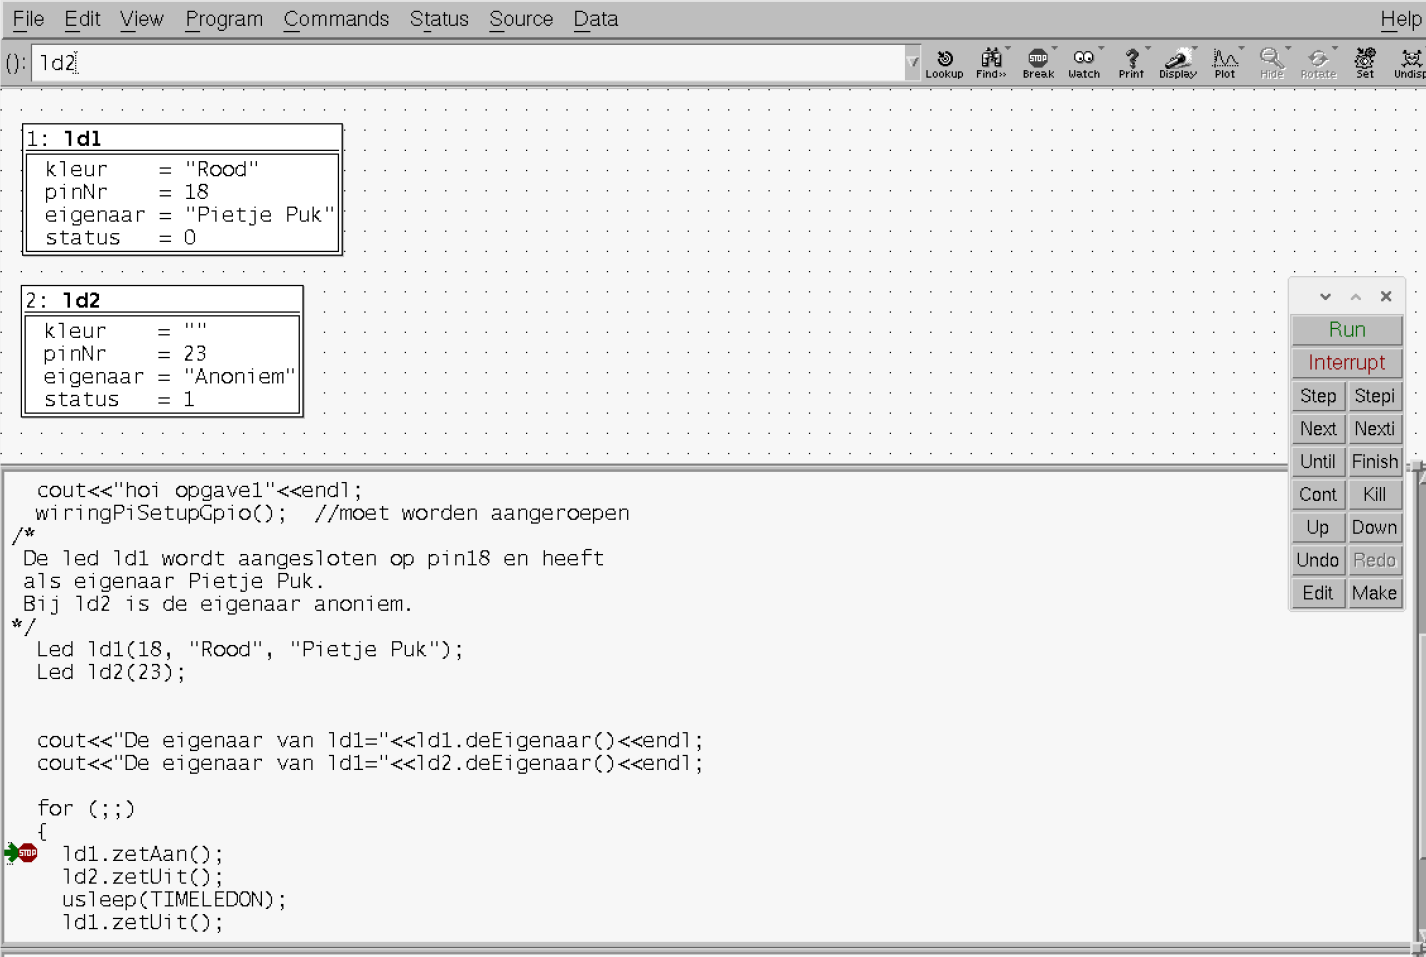
\includegraphics[width=0.9 \linewidth]{figuren/LedDDD}
		 	\centering
		 	\caption{Weergave van twee objecten van de klasse Led.}
		 	\label{fig:dddLeds}
		 \end{figure}
\end{enumerate}
	 \item Maak een screenshot die lijkt op Figuur \ref{fig:dddLeds} alleen met je \textbf{eigen naam} in plaats van ''Pietje Puk'' en upload deze op Brightspace.
	 \item Plaats de screenshot in je portfolio onder hoofdstuk programmeren $\Longrightarrow$ subhoofdstuk \ref{sec:startDDD}. Laat de opdracht aftekenen met onder andere een zichtbaar screenshot.
 
\end{enumerate}

